\section{Grenzwerte}

\subsection{Grenzwert am Beispiel der harmonischen Folge}

\paragraph{Die harmonische Folge}

\[
  a_n = f(n) = \frac{1}{n}  
\]

\[
	\langle a_n \rangle = 1,\ \frac{1}{2},\ \frac{1}{3},\ \frac{1}{4},\ \frac{1}{5},\ \ldots,\ \frac{1}{n}
\]

\begin{figure}[H]
  \centering
  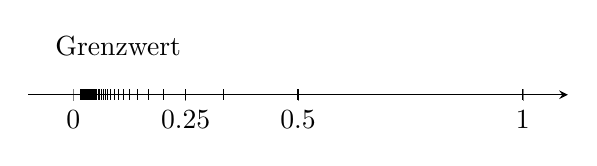
\begin{tikzpicture}
    \begin{axis}[
      % center the x axis
      axis x line=middle,
      % we don't need a y axis line ...
      axis y line=none,
      % ... and thus there is no need for much `height' of the axis
      height=80pt,
      % but `height' also changes `width' which is restored here
      width=\axisdefaultwidth,
      ymin=0,
      ymax=1,
      xmin=-0.1,
      xmax=1.1,
      xtick={0,1/4,1/2,1},
      ]
      \addplot [mark=|] coordinates {
        (1/0,0)(1/1,0)(1/2,0)(1/3,0)(1/4,0)(1/5,0)(1/6,0)
        (1/7,0)(1/8,0)(1/9,0)(1/10,0)(1/11,0)(1/12,0)(1/13,0)
        (1/14,0)(1/15,0)(1/16,0)(1/17,0)(1/18,0)(1/19,0)(1/20,0)
        (1/21,0)(1/22,0)(1/23,0)(1/24,0)(1/25,0)(1/26,0)(1/27,0)
        (1/28,0)(1/29,0)(1/30,0)(1/31,0)(1/32,0)(1/33,0)(1/34,0)
        (1/35,0)(1/36,0)(1/37,0)(1/38,0)(1/39,0)(1/40,0)(1/41,0)
        (1/42,0)(1/43,0)(1/44,0)(1/45,0)(1/46,0)(1/47,0)(1/48,0)
        (1/49,0)(1/50,0)(1/51,0)(1/52,0)(1/53,0)(1/54,0)(1/55,0)
        (1/56,0)(1/57,0)(1/58,0)(1/59,0)(1/60,0)(1/61,0)(1/62,0)
        (1/63,0)(1/64,0) 
        };
      \node[] at (axis cs: 0.1,0.5) {Grenzwert};
    \end{axis}
  \end{tikzpicture}
\end{figure}

\[
  \text{Grenzwert: }\lim_{n \rightarrow \infty} a_n = g = 0
\]

\paragraph{Die harmonische Folge leicht verändert}

\begin{align*}
  a_n &= f(n) = {(-1)}^n + \frac{1}{n} \\
  a_1 &= {(-1)}^1 + \frac{1}{1} = 0 \\
  a_2 &= {(-1)}^2 + \frac{1}{2} = \frac{3}{2} \\
  a_3 &= {(-1)}^3 + \frac{1}{3} = -\frac{2}{3} \\
  a_4 &= {(-1)}^4 + \frac{1}{4} = \frac{5}{4} \\
  a_5 &= {(-1)}^5 + \frac{1}{5} = -\frac{4}{5}
\end{align*}

\begin{figure}[H]
  \centering
  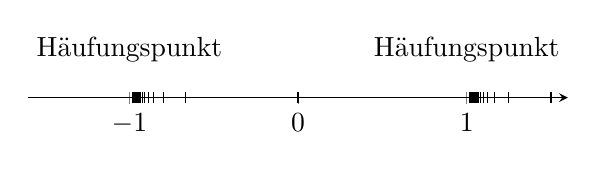
\begin{tikzpicture}
    \begin{axis}[
      axis x line=middle,
      axis y line=none,
      height=80pt,
      width=\axisdefaultwidth,
      ymin=0,
      ymax=1,
      xmin=-1.6,
      xmax=1.6,
      xtick={-1, 0, 1},
      ]
      \addplot [mark=|] coordinates {
        (0,0)(3/2,0)(-2/3,0)(5/4,0)(-4/5,0)(7/6,0)
        (-6/7,0)(9/8,0)(-8/9,0)(11/10,0)(-10/11,0)
        (13/12,0)(-12/13,0)(15/14,0)(-14/15,0)(17/16,0)
        (-16/17,0)(19/18,0)(-18/19,0)(21/20,0)(-20/21,0)
        (23/22,0)(-22/23,0)(25/24,0)(-24/25,0)(27/26,0)
        (-26/27,0)(29/28,0)(-28/29,0)(31/30,0)(-30/31,0)
        (33/32,0)(-32/33,0)(35/34,0)(-34/35,0)(37/36,0)
        (-36/37,0)(39/38,0)(-38/39,0)(41/40,0)(-40/41,0)
        (43/42,0)(-42/43,0)(45/44,0)(-44/45,0)(47/46,0)
        (-46/47,0)(49/48,0)(-48/49,0)(51/50,0)(-50/51,0)
        (53/52,0)(-52/53,0)(55/54,0)(-54/55,0)(57/56,0)
        (-56/57,0)(59/58,0)(-58/59,0)(61/60,0)(-60/61,0)
        (63/62,0)(-62/63,0)
        };
        
        \node[] at (axis cs: -1,0.5) {Häufungspunkt};
        \node[] at (axis cs: 1,0.5) {Häufungspunkt};
    \end{axis}
  \end{tikzpicture}
\end{figure}


\subsection{Definition}

Eine Zahlenfolge \( \langle a_n \rangle \) hat einen Grenzwert \(g\),
wenn es zu einem beliebig kleinen vorgegebenen \(\epsilon > 0\)
eine Zahl \(n_0\) gibt, so dass gilt:

\[
    \mid a_n - g \mid\ < \epsilon, \forall n > n_0
\]

\subsection{Grenzwertsätze}

\begin{align*}
    \langle a_n \rangle \quad \limtoinfty{n} a_n &= \alpha \\
    \langle b_n \rangle \quad \limtoinfty{n} b_n &= \beta
\end{align*}

\begin{enumerate}
    \item \( \limtoinfty{n} (a_n \pm b_n)
        = \limtoinfty{n} a_n \pm \limtoinfty{n} b_n
        = \alpha \pm \beta \)
    \item \( \limtoinfty{n} (a_n \cdot b_n) 
        = \limtoinfty{n} a_n \cdot \limtoinfty{n} b_n
        = \alpha \cdot \beta \)
    \item \( b \neq 0 \text{ für alle } n \in \mathbb{N},
        \beta \neq 0 \text{:} \) \\
        \( \limtoinfty{n} \left(\dfrac{a_n}{b_n}\right)
        = \dfrac{\limtoinfty{n} a_n}{\limtoinfty{n} b_n} \)
    \item \(
        \limtoinfty{n} \sqrt[n]{a_n}
        = \sqrt[n]{\limtoinfty{n} a_n}
        \)
    \item  \(
        \limtoinfty{n} \lambda \cdot a_n
        = \lambda \cdot \limtoinfty{n} a_n
        \)
\end{enumerate}

